\documentclass{llncs}
\usepackage[show]{ed}
\usepackage{calbf}
\usepackage{stex-logo}
\usepackage{amstext,amsmath,amssymb}
\usepackage{xspace}
\usepackage{listings}\lstset{basicstyle=\sf,columns=fullflexible}

% \usepackage{mdframed}
% \newenvironment{boxedquote}{\begin{mdframed}[leftmargin=1cm,rightmargin=1cm]}{\end{mdframed}}

\usepackage{wrapfig,paralist}
\usepackage[hyperref,style=alphabetic,backend=bibtex]{biblatex}
% \addbibresource{kwarcpubs.bib}
% \addbibresource{extpubs.bib}
% \addbibresource{kwarccrossrefs.bib}
% \addbibresource{extcrossrefs.bib}
\addbibresource{kwarc.bib}
\addbibresource{rest.bib}
\def\latexml{{\LaTeX}ML\xspace}
\pagestyle{plain}
\usepackage{tikz}\usetikzlibrary{docicon}

\usepackage{hyperref} \title{System Description: A Semantics-Aware {\LaTeX}-to-Office
  Converter} \author{Lukas Kohlhase and Michael Kohlhase}
\institute{Mathematics/Computer Science\\
  Jacobs University Bremen}
\begin{document} 
\maketitle
\begin{abstract}
  We present a {\LaTeX}-to-Office conversion plugin for \latexml that can bridge the
  divide between publication practices in the theoretical disciplines (\LaTeX) and the
  applied ones (predominantly Office). The advantage of this plugin over other converters
  is that \latexml conserves enough of the document- and formula structure, that the
  transformed structures can be edited and processed further.
\end{abstract}

\section{Problem \& State of the Art}\label{sec:intro}

Technical documents from the STEM (\underline{S}cience, \underline{T}echnology,
\underline{E}ngineering, and \underline{M}athematics) fields augment the text with structured
objects -- images, mathematical/chemical formulae, diagrams, and tables -- that carry
essential parts of the information. There are two camps with different techniques for
authoring documents. The more theoretical disciplines (Mathematics, Physics, and Computer
Science) almost exclusively {\LaTeX}, while the more applied ones (e.g. Life Sciences,
Chemistry, Engineering) use Office Suites almost exclusively. Transforming between these
two document formatting approaches is non-trivial: The {\TeX/\LaTeX} paradigm relies on
in-document macros to ``program'' documents, empowering authors to automate document
aspects and leading to community-supplied domain-specific extensions via {\LaTeX}
packages. Office suites rely on document-styles that adapt visual parameters of the
underlying document markup either document-wide or for individual elements.

This incompatibility of document preparation approaches causes friction in cross-paradigm
collaboration as each camp deems their approach vastly superior and the other's
insufferable. In this paper, we will discuss the transformation from {\TeX/\LaTeX} to
Office documents.

\begin{figure}[ht]\centering
  \begin{tabular}{|c|c|}\hline%|
    copy from PDF & paste (libreoffice)\\\hline
    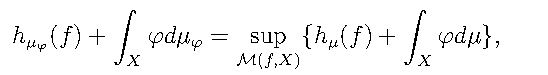
\includegraphics[width=6cm]{mathsnippet} & 
    
\includegraphics[width=5cm]{mathsnippet-libreoffice}\\\hline
  \end{tabular}
\caption{Copy \& Paste in Word Processors}\label{fig:cnp}
\end{figure}

There are several methods to transform papers from {\LaTeX} to an office word
processor. The first method is to just generate a PDF file and then open this file in
Word/LibreOffice. This achieves the goal of looking like the desired PDF document, just in
Office. There are two problems with this route: 
\begin{enumerate}
\item mathematical formulae are not preserved (see Figure~\ref{fig:cnp})
\item even if the result looks OK the results have lost their links (e.g. for
  citations/references or label/ref), or become difficult to edit, because they do not
  conform to the styling system of the word processor.
\end{enumerate}
The fundamental problem is that it converts the appearance of the document and loses
meaning due to macro expansion. This is especially blatant when looking at the math in a
document. Either it is treated as text, with no meaningful way to distinguish between math
and formatted text that happens to contain some mathematical symbols, making automatic
treatment of this kind of math difficult, or it is represented by an image of the relevant
formulae, which makes editing extremely impractical, if not impossible. The same holds true
for references, they are essentially treated as parts of text with a linked number in
front of them, complicating adding new references substantially.

The other way of transforming {\LaTeX} to Word, by transforming the {\LaTeX} source file
directly, avoids these problems. \texttt{latex2rtf}~\cite{latex2rtf:on} is a widely used
system that uses a custom parser to convert a non-trivial fragment of {\LaTeX} to the RTF
format understood by most office systems. The system works well, but coverage is limited
by the {\LaTeX} parser and the aging RTF format.  TeX4ht~\cite{tex4ht:online}, which uses
the {\TeX} parser itself and seeds the output with custom directives that are parsed to
create HTML has a post-processor that generates ODF. Its coverage of {\LaTeX} is unlimited,
but the intermediate format HTML somewhat limits the range of document fragments that can
be generated. 

Here we present a similar approach, only that we extend the backend of the \latexml system
to generate WML -- the file format of MS Word -- and ODT -- that of Libre- and
OpenOffice. Like \texttt{latex2rdf} \latexml directly parses {\LaTeX} source files, but
the coverage of \TeX is complete (including macro definitions) and semantics-preserving
bindings for the most important {\LaTeX} packages are provided. The main difference to
TeX4ht is that \latexml generates an XML representation that is structurally near to the
{\LaTeX} sources and preserves the author-supplied semantics for further processing.

\section{The Office Formats}\label{sec:target}

WML and ODT follow the same architectural paradigm: they are both zip-packaged
directories; their contents and structure differ mainly in media types, XML document
types, and naming. We will use WML in our presentation here and point out differences in
ODT as we go along.

The main content of a WML document -- text, document structure, placement of images,
tables etc. -- is represented by special elements in an XML file
\texttt{document.xml}. All elements contain styling information, usually by referencing a
style element in the file \texttt{style.xml}, which can be modified by adding local
settings in children of the \texttt{properties} child. The other important kind of file
are the \texttt{.rels} files, which are again XML. These files contain
\texttt{relationship} elements, which detail the relations between elements in
\texttt{document.xml} and external resources (e.g. for hyperlinks) or resources in the WML
package (e.g. the image data files of). The WML package additionally contains
miscellaneous XML files; e.g. \texttt{settings.xml}, which is used to make the state of
the word processor applications persistent and \texttt{fonttable.xml}, which contains
extra information about fonts. 

\begin{wrapfigure}r{4.8cm}\vspace*{-3em}
\lstinputlisting[basicstyle=\sf\scriptsize,language=XML]{wmlmath.xml}
\vspace*{-3em}
\end{wrapfigure}
Of special interest here is the representation of mathematical formulae. WML uses a
proprietary XML format for presentation markup together with a variant of {\TeX} markup
that is used for user input. The expression of the left is the --slightly abridged --
representation of $1.5\times 10^7$.  The ODT format treats formulae as external objects;
every single one has a subdirectory in the package which contains a presentation MathML
file (for external communication), a user input file in the venerable StarOffice format,
and an image of the formula (for display in the word processor).

\section{Transformation}\label{sec:trans}

\begin{wrapfigure}r{5.3cm}\scriptsize\vspace*{-2em}
\begin{tikzpicture}[yscale=1.2,xscale=1]
\tikzstyle{doc}=[draw,thick,align=center,color=black,
                 shape=document,minimum width=10mm,minimum height=7mm]
\node[doc] (p) at (-1,3.5) {\texttt{paper.tex}};
\node[doc] (b) at (1,3.5) {\texttt{group.bib}};
\node[doc,dashed] (px) at (-1,2.2) {\texttt{paper.ltxml}};
\node[doc,dashed] (bx) at (1,2.67) {\texttt{group.ltxml}};
\draw[->,thick] (p) -- node[left,near end] (l) {\latexml} (px);
\draw[->,thick] (b) -- (bx);
\draw[->,thick] (bx) -- (l);
\node[doc,dashed] (d) at (-2,1) {\texttt{document.xml}};
\node[doc,dashed] (r) at (0.2,1) {\texttt{relations.xml}};
\node[doc] (s) at (1,.3) {\texttt{styles.xml}};
\draw[->,thick] (px) -- node[left]{XSLT}(d);
\draw[->,thick] (px) -- node[right]{XSLT}(r); 
\node[inner sep=0pt,outer sep=0pt] (z) at (-1,.3) {};
\draw[thick] (d) -- (z);
\draw[thick] (r) -- (z);
\draw[thick] (s) -- (z);
\node[doc] (dx) at (0-1,-.4) {\texttt{paper.docx}};
\draw[->,thick] (z) -- node[left] {zip} (dx);
\draw[dotted] (-3.1,-.1) rectangle (1.9,1.9);
\node at (1.6,1.8) {post};
\end{tikzpicture}
\caption{The Transformation Process}\label{fig:arch}\vspace*{-1em}
\end{wrapfigure}
To create the WML/ODT files we first transform the \texttt{.tex} file to an intermediate
XML-based \textsf{LTXML} format using \latexml. Then we use an XSLT stylesheet to generate
\texttt{document.xml}. For \textsf{LTXML} elements that do not have a direct counterpart
in WML we adapt existing WML elements. For instance, a {\LaTeX} \texttt{element} is
represented by a WML \texttt{p} (``paragraph'') element with a special style
``\texttt{quote}'' we added to \texttt{styles.xml}. This which allows the user to later
semantically work with the document, e.g. by changing all quotes to red.  For WML
formulae, we use a stylesheet supplied by to transform the MathML generated by \latexml to
the WML math format. For ODT formulae we make use of \latexml MathML and image generation.
The other file we generate from the ltxml file using XSLT is \texttt{relations.xml}. The
other supporting files such as images are placed into the correct file structure the
post-processor. As the penultimate step some static files, that don't change depending on
the input document, are also placed into the correct directories. The main file of
interest here is \texttt{styles.xml}, which contains the style information of the
document. We had to create this ourselves to recreate the feel of the PDF files generated
by {\LaTeX}. Finally the documents are zipped to create the WML/ODT file.

The user does not see all these transformation, generation, and packaging steps, given a
{\LaTeX} paper, all she has to do is type 
\begin{quote}\tt
latexmlc paper.tex --destination=paper.docx
\end{quote}
A transformation to ODT can be specified by choosing the destination \texttt{paper.odt}.

\section{Conclusion}\label{sec:concl}
We have presented a \latexml plugin that transforms {\LaTeX} papers into Office documents
in a one-line system call. With the recent web front-end of \latexml, it will be simple to
extend this to a web service. The \latexml Word Processing plugin is public domain and is
available from GitHub at~\cite{LaTeX2Office:github:on}. The conversion makes crucial use
of the fact that \latexml preserves more of the document and formula semantics than other
systems that process \LaTeX documents, this ensures that the core process in the
transformation -- the translation of \latexml XML to Office XML (WML or ODF) has enough
information to generate the respective target document structures. The biggest limitations
of the current transformation are that
\begin{inparaenum}[\em i\rm)]
\item we cannot currently generate the text-based input format (StarMath or the WML {\TeX}
  variant) and 
\item citations and references are only partially converted into the ``semantic'' formats.
\end{inparaenum}
This makes it difficult to edit formulae/references in the respective word processors
after transformation. For ODF formulae, we want to make use of the TeXMaths plugin for
Libreoffice, which uses {\LaTeX} instead of StarMath for user input of formulae -- but
hides it in the comment area of the images which makes handling this more difficult.

In the future we want to develop an office package for \LaTeX, which allows the direct
markup of higher-level structures -- e.g. document metadata in {\LaTeX} documents, so that
it can be transferred to the office documents. Similarly, we want to extend the
transformation to carry over even more semantics from the \stex format into semantically
extended office formats like CPoint or
CWord
%~\cite{Kohlhase:SemanticInteractionDesignDiss:biblatex}
; this would finally give us a
way to cleanly interface the currently {\LaTeX}-based document methods in the KWARC group
to applied STEM disciplines.

\printbibliography
\end{document}


%  LocalWords:  maketitle ednote hline libreoffice includegraphics mathsnippet cnp Hier
%  LocalWords:  einen einfuegen glaube ich docx impl odt Latexml erlaerung eigentlich px
%  LocalWords:  nicht zufrieden hiermit concl printbibliography cience echnology texttt
%  LocalWords:  ngineering athematics latex2rdf tikzpicture yscale xscale tikzstyle bx tt
%  LocalWords:  paper.ltxml group.ltxml ltmxl ltxml stex CPoint CWord ist Trennung und rm
%  LocalWords:  zwischen theoretisch praktisch ganz recht angewandte mathematiker bzw
%  LocalWords:  Physiker benutzen doch auch Libre rels fonttable.xml wrapfigure vspace
%  LocalWords:  lstinputlisting basicstyle scriptsize wmlmath.xml textsf latexmlc
%  LocalWords:  inparaenum TeXMaths
